\documentclass[12pt,letterpaper,noanswers]{exam}
\usepackage[usenames,dvipsnames,svgnames,table]{xcolor}
\usepackage[margin=0.9in]{geometry}
\renewcommand{\familydefault}{\sfdefault}
\usepackage{multicol}
\pagestyle{head}
\header{AM 111 Class 13}{}{Approximating integrals, p.\thepage}
\runningheadrule
\headrule
\usepackage{siunitx}
\usepackage{graphicx} % more modern
\usepackage{amsmath} 
\usepackage{amssymb} 
\usepackage{hyperref}
\usepackage{tcolorbox}
\usepackage{listings}
%\usepackage[numbered,autolinebreaks,useliterate]{mcode}

\usepackage{enumitem}
\def\mbf{\mathbf}
\newcommand{\vc}[1]{\boldsymbol{#1}}
\def\dsst{\displaystyle}
\DeclareMathOperator*{\argmin}{arg\,min} % thin space, limits underneath in displays


\begin{document}
 \pdfpageheight 11in 
  \pdfpagewidth 8.5in

\noindent 

\section*{Preliminaries}

\begin{itemize}
\itemsep0pt
\item There is a problem set due Friday.
\item There is a skill check in the next class.
\end{itemize}


\noindent\textbf{Big picture}

Today: Approximating $\int_{a}^{b}f(x)dx$.

\vspace{0.2cm}
\hrule
\vspace{0.2cm}

\noindent \textbf{Skill check practice}

 Find the degree of precision of the following approximation for $\displaystyle\int_{-1}^1 f(x)\ dx$:
% $f(1)+f(-1)$, 
%$\dfrac{2}{3}[f(-1)+f(0)+f(1)]$, %$f\left(\dfrac{1}{\sqrt{3})\right) + f\left(\dfrac{1}{\sqrt{3})\right)$

$\displaystyle\int_{-1}^1 f(x)\ dx\approx 2f(0)$.

\emph{The following information may be helpful}
\[\int_{-1}^1 1\ dx = 2, \int_{-1}^1 x\ dx = 0, \int_{-1}^1 x^2\ dx = \frac{2}{3}, \int_{-1}^1 x^3\ dx =0, \int_{-1}^1 x^4\ dx = \frac{2}{5}\]



\vspace{0.2cm}
\hrule
\vspace{0.2cm}

\noindent \textbf{Skill check solution}

The degree of precision is the greatest integer $k$ for which all polynomials of degree $k$ or less are integrated exactly by the method.

degree 0: For $f(x) = c_0$, $2f(0) = 2c_0$ and $\int_{-1}^1 c_0\ dx = 2c_0$  so this is exact for $f$ constant.

degree 1: For $f(x) = c_1 x$, $2f(0) = 0$ and $\int_{-1}^1 c_1 x\ dx = 0$ so this is exact for $f$ linear.

degree 2: For $f(x) = c_2 x^2$, $2f(0) = 0$ and $\int_{-1}^1 c_2 x^2\ dx = \frac{2}{3}c_2$, which does not match.

The degree of precision is $1$.


\vspace{0.2cm}
\hrule
\vspace{0.2cm}


\section*{Numerical Integration}


\subsection*{Newton-Cotes formulas}

\begin{enumerate}[resume=classQ]
\item Assume $f(x) \in C^2[a,b]$.  $C^2$ means there is continuity of $f, f', f''$ on the interval.  

Use $x_0 = a, x_1 = b$ as nodes for Lagrange interpolation, with $y_k = f(x_k)$.
\begin{parts}
    \item Write down $p_1(x)$, the first-degree polynomial interpolating $f$ at $x_0, x_1$.  
    \vspace{1cm}
    \item Find $\int_a^b p_1(x)dx$ as an approximation to $\int_a^b f(x)dx$.
    \vspace{1in}
    \item What quadrature rule is this?
    \vspace{0.5cm}
\end{parts}
\end{enumerate}



% \begin{enumerate}[resume=classQ]
% \item We will find the error for the trapezoid rule.
% \begin{parts}
% \item
% Use the interpolation error formula to write an integral expression for the error in the trapezoid rule.
% \vspace{1cm}

% \item What is the sign of $(x-a)(x-b)$ for $x\in [a,b]$?
% \vspace{1cm}
% \item Recall the mean value theorem for integrals: Let $f:[a,b]\rightarrow\mathbb{R}$ be continuous, and $g$ an integrable function that does not change sign on $[a,b]$. Then there exists $c\in(a,b)$ such that $\displaystyle\int_a^b f(x)g(x) dx = f(c)\int_a^b g(x)dx$.

% Use this theorem to remove $f''(c)$ from within the integral, and then evaluate the integral.

% \emph{I suggest using integration by parts: Set $u = x-a, dv = (x-b)dx$.}
% \vspace{1in}

% \end{parts}
% \end{enumerate}
%You should find that the error is cubic in the size of the interval and proportional to the second derivative of $f$.
\begin{enumerate}[resume=classQ]
\item For any $f(x)$ that is linear in $x$, what will be the error when using the trapezoid rule?
\vspace{1cm}
\end{enumerate}



\begin{enumerate}[resume=classQ]
    \item Let $p_2(x) = y_0L_1(x) + y_1L_2(x)+y_2L_3(x)$ where $x_0 = a, x_1 = (a+b)/2, x_2 = b$ and $y_k = f(x_k)$.  
    
    $\displaystyle\int_a^b p_2(x) = A_0 y_0 + A_1 y_1 + A_2 y_2$.  You can find $A_0, A_1, A_2$ by integrating $L_1, L_2, L_3$.  Instead of integrating, use the integral information in the caption of the figure below (parts b and c) to find $A_0, A_1, A_2$.  Note that $h = (b-a)/2$.
\end{enumerate}


    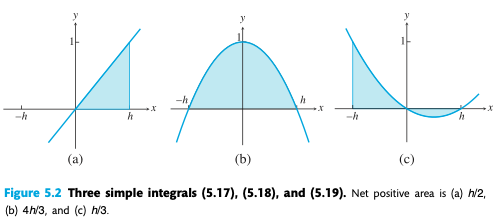
\includegraphics[width=0.6\textwidth]{img/Class12Sauerintegrals.png}
\begin{enumerate}[resume=classQ]
%     \item The \textbf{method of undetermined coefficients} is another option for finding $A_0, A_1, A_2$.
%     \begin{parts}
%     \item For $f(x)$ a constant, linear, or quadratic polynomial, $\int_a^b f(x)dx = A_0 y_0 + A_1 y_1 + A_2 y_2$ is exact.
    
%     Let $f(x) = 1$.  Use $\int_a^b 1\ dx = A_0  + A_1 + A_2 $ to find an equation for $A_0+A_1+A_2$ in terms of $a$ and $b$.
%     \vspace{1in}
%     \item Repeat this for $f(x) = x$ and $f(x) = x^2$ to generate two more equations in terms of $A_0, A_1, A_2$ and $a,b$.
%     \vspace{2in}
%     \item Write your linear system as a matrix equation.
%     \vfill
%     \end{parts}
    
% The solution to the system is $A_0 = A_2 = \dfrac{b-a}{6}$, $A_1 = 4\dfrac{b-a}{6}$.
\end{enumerate}



\begin{enumerate}[resume=classQ]
    \item Show that the degree of precision for Simpson's rule is $3$.
    
    To do this, we need to show that $\int_a^b 1\ dx$, $\int_a^b x\ dx$, $\int_a^b x^2\ dx$, $\int_a^b x^3\ dx$ are all integrated exactly by Simpson's rule.

$\int_a^b 1\ dx$, $\int_a^b x\ dx$, $\int_a^b x^2\ dx$ are integrated exactly by construction of the rule, so what is left to show is that $\int_a^b x^3\ dx$ is integrated exactly.
    \begin{parts}
    \item One way to do this is to shift your integral.  Find $k$ such that $\int_a^b x^3 dx = \int_{-h}^h (x+k)^3 dx$.
    \vspace{1cm}
    
    \item Expanding, $(x+k)^3 = x^3 + q(x)$ where $q(x)$ is a quadratic function.  
    
    $\int_a^b x^3 dx = \int_{-h}^h (x+k)^3 dx = \int_{-h}^h x^3 dx  + \int_{-h}^h q(x) dx$
    
    Provide an argument for why each term of the final expression is zero.
    \vspace{1.5in}
    
    
    
    \end{parts}
    
\end{enumerate}

\subsection*{Composite rules}

\begin{enumerate}[resume=classQ]
    \item In a single panel, the error from the Trapezoid rule is given by $-\frac{1}{12}h^3f''(c_k)$ with $x_{k-1}<c_k<x_k$.
    \begin{parts}
    \item Find an expression for the sum of the error over all $m$ panels (use summation notation).
    
\vspace{1in}
\item The generalized intermediate value theorem says that for $f$ continuous on $[a,b]$, $c_k$ points in $[a,b]$, and weights $w_1, ..., w_m>0$, there exists a number $c$ between $a$ and $b$ such that $w_1f(c_1)+...+w_mf(c_m) = (w_1+...+w_m)f(c)$.  Use this theorem to write your expression as $f''(c)$ times a constant.  Write the constant in terms of $m$ and $h$.
\vspace{1in}
\item Is the error you found equal to $- (b-a)\frac{h^2}{12}f''(c)$?
\vspace{1cm}
    \end{parts}
\end{enumerate}

The error in the Trapezoid rule is proportional to $f''$ and to $h^3$.

The error in the composite Trapezoid rule is proportional to $f''$ and to $h^2$.

See the reading for details on composite Simpson's rule.

% \begin{enumerate}[resume=classQ]
% \item For composite Simpson's rule, let each panel be length $2h$.  Use the grid $a = x_0 < x_1 < ... < x_{2m-1}<x_{2m}$.
% \begin{parts}
% \item For $a = x_0, b = x_2$, Simpson's rule can be written $\int_a^b f(x)dx \approx \frac{h}{3}(y_0 + 4y_1 + y_2)$.

% The composite rule is of the form \[\frac{h}{3}\left[y_0 + A \sum\limits_{k=1}^m y_{2k-1} + B\sum\limits_{k=1}^{m-1}y_{2k} + y_{2m}\right].\]

% Find $A$ and $B$.
% \end{parts}
% \end{enumerate}

\subsection*{Open vs closed formulas}

\begin{enumerate}[resume=classQ]
    \item To approximate $\displaystyle\int_a^b f(x)dx$, let $x_0 = a, x_1 = b$, $h = b-a$.  Set $w = x_0 + h/2$ (the midpoint of the interval).
    \begin{parts}
    \item Find the degree $1$ Taylor expansion of $f(x)$ about the midpoint $w$.  Do this exactly, so include the remainder term (it is $\frac{1}{2}(x-w)^2f''(c)$.
    \vspace{1in}
    \item Integrate both sides from $a$ to $b$.
    
    Note that $f'(w)$ is a constant.  Use the mean value theorem for integrals to remove $f''(c)$ from the integral.
    \vspace{1in}
    
    \end{parts}
This generates the \textbf{midpoint rule} for approximating an integral.
\end{enumerate}



%     \fbox{
%     \begin{minipage}{15cm}
%       \subsection*{Composite Midpoint Rule}
%       Given a function $f(x) \in C^4(a,b)$ and equally spaced
%       points $a=x_0<x_1<\cdots<x_{2m}=b$, $x_{i+1}-x_i = h$,
%       \begin{equation}
%         \int_a^b f(x) \, dx = h \sum_{i=1}^m f\left(\frac{x_{i-1} + x_i}{2}\right) + \frac{(b-a)h^2f''(\xi)}{24}.
%       \end{equation}
%     \end{minipage}}

% \pagebreak

% \subsection*{Adaptive Quadrature}

% \pagebreak

% \been

% \item Read the adaptive quadrature algorithm in the book (\S5.4) and implement it to estimate:

% \beit
% \item $\int_{-1}^1   2\sqrt{1-x^2} dx$
% \item $\int_{-1}^1   1+\sin(e^{3x}) dx$
% \enit

% \enen



%
%\subsection*{Romberg Integration}
%
%\been
%
%\item[4.] Romberg integration uses the composite trapezoid rule with successively
%smaller stepsizes $h$.
%
%\been
%\item {\bf Romberg Integration (First Column)}
%
%Define stepsizes $h_j$ such that each successive stepsize is half the
%previous stepsize:
%\begin{align*}
%h_1 &= b-a \\
%h_2 &= (b-a)/2 \\ 
%h_3 &= (b-a)/4 \\
%& \vdots \\
%h_j&=\frac{1}{2^{j-1}}(b-a).
%\end{align*}
%
%The first column of Romberg integration, $R_{j1}$, is the composite
%trapezoid rule applied to the function on $[a,b]$ with stepsize $h_j$.  Write down the formula for the first few elements of the first column:
%
%\vfill
%
%\begin{align*}
%R_{11} &= \blank{3in} \\
%& \\
%R_{21} &= \blank{3in} \\
%& \\
%R_{31} &= \blank{3in}
%\end{align*}

%\pagebreak
%
%The second column applies Richardson extrapolation to the 1st column
%$R_{j1}$.  Write down the results for the second column.  What is $R_{22}$?
%
%\vfill
%
%\begin{align*}
%R_{22} &= \frac{2^2 R_{21} - R_{11}}{3} = \blank{3in} \\
%& \\
%R_{32} &= \frac{2^2 R_{31} - R_{21}}{3} = \blank{3in}
%\end{align*}
%
%\item Calculate $R_{11}$, $R_{21}$, and $R_{22}$ for $\dsst{\int_0^4 x^2 \, dx}$.
%
%\vfill
%
%\pagebreak
%
%\item The third column applies Richardson extrapolation to the second column.
%Because the second column is composite Simpson's rule, it is 4th order in $h$:
%\begin{align*}
%R_{33} &= \frac{4^2 R_{32} - R_{22}}{4^2-1} \\
%R_{43} &= \frac{4^2 R_{42} - R_{32}}{4^2-1} \\
%& \vdots \\
%R_{j3} &= \frac{4^2 R_{j2} - R_{j-1,2}}{4^2-1}
%\end{align*}
%
%\item This pattern perpetuates
%$$
%R_{jk} = \frac{4^{k-1} R_{j,k-1} - R_{j-1,k-1}}{4^{k-1}-1} 
%$$
%
%\enen
%
%\item[5.] Computer Examples
%\been
%
%\item Estimate $\dsst{\int_{-1}^1 2\sqrt{1-x^2} \, dx}$.
%
%\vspace{1cm}
%
%\item Estimate $\dsst{\int_{-1}^1 1 + \sin{e^{3x}} \, dx}$.
%
%\vspace{1cm}
%
%\enen
%
%\enen



\subsection*{Gaussian quadrature (following Sauer \S5.5)}


\begin{enumerate}[resume=classQ]
    \item Consider $I = \int_a^b f(x)dx$.  Let $g(x) = f(x+h+a)$, $h = (b-a)/2$.  $I = \int_{-h}^h g(x) dx$.
    
        $\int_{-h}^h g(x) dx \approx c_1 g(x_1) + c_2 g(x_2)$.  We would like to $c_1, c_2, x_1, x_2$ to maximize the degree of precision of this method.  
        
        With four unknowns that we can set, the method should be exactly correct for $g(x) = 1, x, x^2, x^3$ (degree of precision of $3$).
    \begin{parts}
\item Assuming a degree of precision of $3$, find four equations that are satisfied by $c_1, c_2, x_1, x_2$.
\vspace{1.5in}
\item This is a system of nonlinear equations.  Make an effort to find a solution to the system (you might use that $c_1x_1 = -c_2x_2$).  \emph{It is typically difficult to find a solution to a nonlinear system}.

\vfill

\item If you were to use $n$ points instead of $2$ points, how many unknowns would you have?  What degree of precision is possible (assuming the system you generate has a solution)?
\end{parts}
\end{enumerate}
\eject


\begin{enumerate}[resume=classQ]
\item You are using an $n$ point quadrature method.  Assume you have been told to use points $x_1, x_2, ..., x_n$ (where the $x_k$ values are given to you) to create an interpolating polynomial.

Let $L_k(x)$ be the basis functions for Lagrange interpolation.  

Write an expression to find $c_k$ where $\displaystyle\int_{-h}^h g(x) dx \approx \sum\limits_{k=1}^n c_k f(x_k)$.
\vspace{1in}

\end{enumerate}

\begin{enumerate}[resume=classQ]
\item %Let $P(x)$ be a polynomial of degree at most $2n-1$.

(What are orthogonal polynomials?)

Let $\{p_0(x),p_1(x),...,p_k(x),...,p_n(x)\}$ be a set of orthogonal polynomials on the interval $[-h,h]$ with $p_k$ of degree $k$.
\begin{parts}
\item Two polynomials, $f(x)$ and $g(x)$, are orthogonal on an interval $[-h,h]$ if 

$\displaystyle\int_{-h}^h f(x)g(x)dx = 0$.  Show that $p_0(x) = 1$ and $p_1(x) = x$ are orthogonal on $[-1,1]$.
\vspace{1in}
\item Let $p_2(x) = x^2 + c$.  Find $c$ so that $p_2(x)$ is orthogonal to $p_1(x)$ and to $p_0(x)$.
\vspace{1in}

\end{parts}
\end{enumerate}

\begin{enumerate}[resume=classQ]
    \item Set the $n$ values of $x_i$ to be the roots of $p_n(x)$.  Using polynomial long division, $x^j = S(x)p_n(x) + R(x)$ where $j \leq 2n-1$, $S(x)$ is degree at most $n-1$ and $R(x)$ is the remainder so also degree at most $n-1$.
    \begin{parts}
    \item Write $S(x) = \sum\limits_{i=1}^{n-1} a_i p_i(x)$.  How do you know it is possible to write $S(x)$ in this way?
    \vspace{1cm}
    \item Find $\int_{-1}^1 S(x)p_n(x)dx$.  \emph{By orthogonality, you know $\int_{-1}^1 p_i(x)p_n(x)dx$.}
    \vspace{1in}
 
 You should find that $\int_{-1}^1 x^j dx = \int_{-1}^1 R(x)dx$.  $R(x)$ is of degree $n-1$ or less, so an interpolating polynomial on $n$ points will exactly match it.  
 
 \item Argue that $\int_{-1}^1 x^j dx$ is equal to the quadrature rule applied to $R(x)$, so $\sum\limits_{i=1}^n c_i R(x_i)$.
 \vspace{1cm}
 
 \item Now consider the quadrature rule applied to $x^j = S(x)p_n(x) + R(x)$.  For $x_i$ the roots of $p_n(x)$ simplify $S(x_i)p_n(x_i) + R(x_i)$.
 \vspace{1cm}
    \end{parts}
\end{enumerate}


\subsection*{Adaptive quadrature}

\begin{lstlisting}[basicstyle=\small]
% From Sauer: program 5.2 Adaptive Quadrature
% Computes approximation to definite integral
% Inputs: Matlab function f, interval [a0,b0], 
%   error tolerance tol0
% Output: approximate definite integral
function sum = adapquad(f,a0,b0,tol0)
sum=0; 
n=1; 
a(1)=a0; 
b(1)=b0; 
tol(1)=tol0; 
app(1)=trap(f,a,b);
% n is current position at end of the list
while n>0           
  c = (a(n)+b(n))/2;
  oldapp = app(n);
  app(n) = trap(f,a(n),c);
  app(n+1) = trap(f,c,b(n));
  if abs(oldapp-(app(n)+app(n+1))) < 3*tol(n)
    % success
	sum = sum + app(n) + app(n+1);
	% done with interval
	n = n-1;                         
  else
    % divide into two intervals
    % set up new intervals
	b(n+1)=b(n); 
	b(n)=c;
	a(n+1)=c;
	tol(n)=tol(n)/2; tol(n+1)=tol(n);
	% go to end of list, repeat
	n=n+1;                         
  end
end

function s=trap(f,a,b)
s = (f(a)+f(b))*(b-a)/2;

\end{lstlisting}

% \begin{enumerate}[resume=classQ]
% \item Let $I = \displaystyle\int_0^1 x^2 dx$.  For your reference, $I = 1/3$.
% \begin{parts}
% \item Call \texttt{adapquad(f,0,1,0.01)}.  In the first column, follow each of the variables on the first pass through the loop.  As a variable updates, cross out the old value and write the new one.

% Trace the program to line 33 for the first time through the loop.

% Then trace again for the second pass through the loop.

% \begin{tabular}{l|p{5cm} | p{5cm}| c}
% variable & time 1 & time 2 & ...\\
% \hline
% & && \\
% sum & && \\
% & &&\\
% n & && \\ & &&\\
% a & && \\ & &&\\
% b & && \\ & &&\\
% tol & & &\\ & &&\\
% app & && \\ & &&\\
% c & && \\ & &&\\
% oldapp & && \\%& &&\\

% \end{tabular}

% \item What does this code do?  Why is the method called \emph{adaptive}?
% \vspace{1in}

% \end{parts}
% \end{enumerate}

\end{document}